\documentclass[]{article}

\usepackage{float}
\usepackage{svg}
\usepackage{amsmath}
\usepackage{parskip}
\usepackage[colorlinks=true, allcolors=blue]{hyperref}
\usepackage[margin=2cm]{geometry}
\usepackage{amsthm}
\usepackage{dsfont}
\usepackage[many]{tcolorbox}
\usepackage{amsfonts}
\usepackage{listings}
\usepackage{color}
\usepackage{braket}
\usepackage{mathtools}
\usepackage{todonotes}
\usepackage{kpfonts}
\usepackage[labelfont=bf, textfont=it]{caption}
\usepackage{blindtext}
\usepackage[]{multicol}
\usepackage[]{subfig}

\usepackage{titlesec}

% \titleformat*{\section}{\large\bfseries}
% \titleformat*{\subsection}{\bfseries}
% \titleformat*{\subsubsection}{\bfseries}
% \titleformat*{\paragraph}{\bfseries}
% \titleformat*{\subparagraph}{\bfseries}

\titleformat{\section}
{\normalfont\large\bfseries}{\thesection}{0.4em}{\vspace{-0.2em}}
\titleformat{\subsection}
{\normalfont\bfseries}{\thesubsection}{0.4em}{}
\titleformat{\subsubsection}
{\normalfont\normalsize\bfseries}{\thesubsubsection}{0.4em}{}
\titleformat{\paragraph}[runin]
{\normalfont\normalsize\bfseries}{\theparagraph}{0.4em}{}
\titleformat{\subparagraph}[runin]
{\normalfont\normalsize\bfseries}{\thesubparagraph}{0.4em}{}


% biblatex
\usepackage[style=numeric, sorting=none]{biblatex}
\addbibresource{bib.bib}

% fancy itemize
\usepackage[inline]{enumitem}
\setitemize{noitemsep,topsep=0pt,parsep=0pt,partopsep=0pt}

% \abs for absolute value
\DeclarePairedDelimiter{\abs}{\lvert}{\rvert}
\DeclarePairedDelimiter{\norm}{\lvert\lvert}{\rvert\rvert}

\svgpath{img/svg/}
\graphicspath{{img/svg_out/}{img/png}}

\definecolor{codegreen}{rgb}{0,0.6,0}
\definecolor{codegray}{rgb}{0.5,0.5,0.5}
\definecolor{codepurple}{rgb}{0.58,0,0.82}
\definecolor{backcolour}{rgb}{0.96,0.96,0.96}
\definecolor{codeblue}{rgb}{0, 0.1, 0.9}

\lstset{
  backgroundcolor=\color{backcolour},
  commentstyle=\ttfamily\color{codegreen},
  keywordstyle=\color{codeblue},
  numberstyle=\tiny\ttfamily\color{codegray},
  stringstyle=\color{codepurple},
  basicstyle=\ttfamily\footnotesize,
  breakatwhitespace=false,
  breaklines=true,
  captionpos=b,
  keepspaces=true,
  %numbers=left,
  numbersep=5pt,
  showspaces=false,
  showstringspaces=true,
  showtabs=false,
  tabsize=2
}

% Fancy abstract
\renewenvironment{abstract}
{
\noindent \rule{\linewidth}{.5pt}
\begin{quote}
\par{\bfseries \abstractname.}
}
{
\end{quote}
\medskip\noindent \rule{\linewidth}{.5pt}
}

\title{%
  \huge \textbf{Efficient direct lighting calculation for area lights with light portals}\\
  \vspace{0.4cm}
  \Large J. Romeu Huidobro\\
  \vspace{0.3cm}
  \large Supervisors:\; M. van de Ruit, E. Eismann\\
  \vspace{0.3cm}
  EEMCS, Delft University of Technology, The Netherlands
  \vspace{-0.8cm}
}
\author{}
\date{}

\begin{document}

\newcommand{\from}[0]{\leftarrow}

\maketitle

\begin{abstract}
  \blindtext[1]
\end{abstract}

\begin{multicols*}{2}
  

\section{Introduction}
\label{sec:intro}

Physically-based Monte Carlo light transport algorithms create photorealistic imagery with applications ranging from videogames to architecture visualization. While they can deliver accurate illumination, their most significant limitation is their high computational demands. 

Direct lighting is often one of the most significant components, so most rendering algorithms compute direct illumination separately, allowing for more effective light sampling. Direct lighting is computed by explicitly casting shadow rays from the shading point to the light sources. The probability distribution function (PDF) from which the shadow ray directions are sampled can have a high impact on the convergence rate of the scene. For example, consider a scene with a lamp occluded by a lampshade, all of the shadow rays blocked by the lampshade will have no contribution to the final image and are thus wasted sampling effort.

One widely used technique for sampling direct lighting from environment lights is \emph{light portals}. These are artist-specified regions which indicate an opening to the environment light. This information is then used during rendering to prioritize sampling the directions that go through the portal. Our contribution is extending the idea of light portals to accelerate the sampling of partially occluded area lights by repurposing concepts from shadow volume calculations.

We begin by reviewing Monte Carlo techniques for direct lighting calculations and provide an overview of existing use cases and sampling strategies for light portals (\autoref{sec:background}). Next, we expand on the details of our method (\autoref{sec:method}) and its implementation into an existing path tracer (\autoref{sec:implementation}). Lastly, we evaluate our portal sampling strategy against light sampling (\autoref{sec:results}), and discuss the results (\autoref{sec:discussion}) before concluding and giving final remarks (\autoref{sec:conclusion}).

\section{Background and related work}
\label{sec:background}

\paragraph*{The Light Transport Equation} 
The light transport equation (LTE) \cite{kajiyaRENDERINGEQUATION1986} is a recursive integral over radiometric quantities (reference), which governs our approximation of light transport.

\begin{equation}
  \begin{aligned}
  L_o(p, \omega_o) &= L_e(p, \omega_o)\\
  &+ \int_{\Omega} f(p, \omega_o, \omega_i) L_o(p, \omega_o, \omega_i) \abs{\cos\theta_i} d\omega_i,
  \end{aligned}
\end{equation}

The equation states that the exitant radiance at point $p$ in direction $\omega_o$ is equal to the emitted radiance at that point and direction plus the portion of the incident light on $p$ that gets reflected towards $\omega_o$.

\paragraph{The direct lighting integral} 

Repeatedly unfolding the recursive call, the LTE can be reformulated into the path-integral formulation \cite*{veachROBUSTMONTECARLO} which separates the contributions of each path length into separate terms. This reformulation allows us to calculate direct and indirect independently. , The direct lighting term is the one we are concerned with evaluating in this paper, and it is given by the integral:

\begin{equation}
  \int_{\Omega} f(p, \omega_o, \omega_i) L_d(p, \omega_i) \abs{\cos\theta_i} d\omega_i,
\end{equation}

where $L_d$ is the \emph{direct} radiance from direction $\omega_i$, $f$ is the Bidirectional Scattering Function (BSDF) and the cosine term accounts for Lamberts law.

\paragraph*{Monte Carlo Integration}
This integral cannot be solved analytically in general, thus we use \emph{Monte Carlo integration} as a means to numerically estimate it. To compute this estimate, we need to sample $N$ directions $\omega_i$ and apply the Monte Carlo estimator \cite{L1996MCTAOFPBR}:

\begin{equation}
  \frac{1}{N} \sum_{i=1}^N \frac{f(p, \omega_o, \omega_i) L_d(p, \omega_r) \abs{\cos\theta_i}}{p(\omega_i)}
\end{equation}

To reduce variance, we can use \emph{importance sampling} to choose the directions $\omega_i$ from a probability density function PDF similar to the integrand. However, when deciding on a distribution to sample from, its clarifying that we are \emph{not} after the distribution providing the lowest variance for a given number of samples, but instead the distribution providing the lowest variance for a given amount of time \cite{shirleyMonteCarloTechniques1996}, thus an effective sampling strategy may be worse than an ineffective one if the latter can be sampled more efficiently.

The most common sampling technique is to choose a light to be sampled for based on a precomputed PDF over the light sources in the scene \cite{shirleyMonteCarloTechniques1996}, weighted based on one or more heuristics such as light power (emitter sampling citations), and then using multiple importance sampling \cite{veachROBUSTMONTECARLO} to draw samples from to the PDF of the BSDF and the light's solid angle, which are then combined according to the contribution of each sample. This approach, however, ignores the visibility of the light source when drawing the samples, which can lead to high variance in scenes where the light is partially occluded, producing many blocked shadow rays.

\paragraph{Light portals}
\emph{Light portals} are artist-specified regions in the scene which indicate an opening to an environment light, such as a window in an interior scene. During rendering, the portal is then used to focus the environment light sampling to only those directions visible through the portal. They are highly effective for accelerating convergence in many scenes and are implemented in several production renderers such as Cycles \cite{LightSettingsBlender} and Renderman \cite{PxrPortalLight}.

The portal area is typically sampled uniformly, although more advanced portal sampling strategies exist \cite{ogakiGeneralizedLightPortals2020}\cite{bitterliPortalMaskedEnvironment2015}. Nonetheless, these sampling strategies are designed for sampling \emph{environment lights}, and several challenges and opportunities are presented when applying the same technique to area lights. Unlike area lights, environment lights extend across the whole scene, so any direction sampled through the portal will also be directed to the environment. For this reason, existing portal sampling strategies are unsuitable for area lights.
\section{Method}
\label{sec:method}

We now present our method. We begin by explaining how the portal is represented and incorporated into the light distribution for a scene with a single light and a single portal. Next, we give an effective yet slow sampling strategy and show how it can be made more efficient by repurposing ideas from shadow calculations. Lastly, we generalize the provided method to multiple portals and multiple lights.

\subsection{Sampling a single light portal}

Consider a simple scene containing a single light source covered by a lampshade (\autoref{fig:simplescene}). The core idea behind our method is to have the artist include the geometry of the opening to the light source as a "portal" in the scene description. This portal is then incorporated into the light distribution of the scene. When constructing the light distribution, the portal is prioritized for points in front of it and never sampled for points behind it.

\begin{figure}[H]
  \def\svgwidth{0.9\columnwidth}
  \input{img/svg_out/simplescene.pdf_tex}
  \caption{Simple scene (left) showing the region behind and in front of the portal. As well as an ilustration of the light distribution for the scene}
  \label{fig:simplescene}
\end{figure}

\subsection{Sampling the portal}
\label{sec:proj-sampling}

In  (background), we explained why uniformly sampling the portal area is not a good strategy when using light portals with area lights. If we want to only sample directions which go through the portal and are facing the light, the region that needs to be sampled is the intersection of the solid angles subtended by the light source and the light portal. 

This region can be sampled by projecting the light source from the perspective of the shading point onto the portal and then clipping the projected region to the portal bounds \cite{sutherlandReentrantPolygonClipping1974}.

\begin{figure}[H]
  \centering
  \def\svgwidth{0.6\columnwidth}
  \input{img/svg_out/projection.pdf_tex}
  \caption{Projecion sampling. The light (yellow) is projected onto the portal-plane (blue) and clipped to the portal bounds. Samples are then drawn from the clipped region (green).}
  \label{fig:projection}
\end{figure} 

This sampling strategy is effective per sample but much slower than light sampling or portal sampling. In the next section, we show how some additional geometry allows us to restrict the use of this sampling strategy to the points where it provides the most significant advantage over more efficient alternatives.

\subsection{Thinking in terms of shadows}
\label{sec:antishadow}

An interesting way to think about light portals is to consider the shadow that the portal would cast if we were to replace it with an occluder. The area in front of the occluder can then be separated into four regions. The \emph{umbra}, \emph{penumbra} and \emph{antumbra} of the shadow, as well as the region out of shadow\cite{hasenfratzSurveyRealtimeSoft2003}. These regions are defined as: 

\begin{itemize}
  \item The \textbf{umbra} (hard shadow) is the portion of the shadow where the occluder blocks all direct paths to the light source.
  \item The \textbf{penumbra} (soft shadow) is the portion of the shadow where some but not all direct paths to the light are occluded.
  \item If the occluder is smaller than the light, the umbra will converge, forming the \textbf{antumbra}, which is the portion of the penumbra where the occluder is directly in front of the light.
  \item The \textbf{region outside of shadow} is the area where none of the paths to the light is occluded.
\end{itemize}

Nonetheless, the portal is not an occluder, but instead precisely the opposite, as it indicates an \emph{opening} to the light. Thus, these same regions take on a new meaning when we treat them from the portal's perspective. The portal-equivalent regions are:

\begin{itemize}
  \item The \textbf{anti-umbra} is the region where all direct paths to the light go through the portal.
  \item The \textbf{anti-penumbra} is the region where some but not all paths to the light go through the portal.
  \item The \textbf{anti-antumbra} is the region where the portal is directly in front of the light but does not fully cover it.
  \item The region \textbf{outside of the antishadow} is the area where none of the paths from the shading point to the light to the light pass through the portal
\end{itemize}

\begin{figure}[H]
  \centering
  \subfloat[2D representation of shadow and antishadow regions.]{
  \def\svgwidth{0.8\columnwidth}
  \input{img/svg_out/antishadow.pdf_tex}
  }
  \\
  \subfloat[View of the light and portal from the point of view of the shading point, in different regions of the portal antishadow.]{
  \def\svgwidth{0.7\columnwidth}
  \input{img/svg_out/antishadow-pov.pdf_tex}
  }
  \label{fig:antishadow}
  \caption{Two-dimensional representation of the regions of a shadow. If we replace the occluder with a light portal, the same geometric volumes take different roles.}
\end{figure}

Returning to our problem of sampling the light going through a portal, having an idea of which region of the antishadow the shading point is in can be used to choose a sampling strategy. Firstly, if the shading point is  \textbf{outside of the antishadow}, there is no need to do any sampling whatsoever, as there are no direct paths through the portal that reach the light. Thus if the shading point is in this region, we can simply return zero without any computation.

If the shading point is in the \textbf{anti-umbra}, all direct paths to the light go through the portal, so visibility is guaranteed. Thus, the optimal sampling strategy is to sample the light source itself. Conversely, when the shading point is in the \textbf{anti-antumbra}, all of the paths through the portal hit the light, making portal sampling the optimal strategy. Figure (antumbra b) gives a good intuition on why this works.

Lastly, points in the \textbf{anti-penumbra} are more complex, as some but not all direct paths to the light go through the portal. In this case, we resort to using the effective, but slow projection sampling method explained in \autoref{sec:proj-sampling}. 

Returning to the simple scene from figure \autoref{fig:simplescene}, we can now partition the space further by including the antishadow volumes. Now, we add the sampling strategies discussed above to the light distribution, weighing the PDF of each strategy based on which region of the antishadow the shading point is contained in.

\begin{figure}[H]
  \def\svgwidth{0.9\columnwidth}
  \input{img/svg_out/simplescene-antishadow.pdf_tex}
  \label{fig:simplescene-antishadow}
  \caption{Simple scene employing antishadow volumes to weight the choice of sampling strategy depending on the location of the shading point.}
\end{figure}

In doing this, we restrict the slow projection sampling technique to only the points in the anti-penumbra and use faster strategies for shading points where there is no additional benefit gained by projecting.

\subsection{Computing the antishadow regions}

In \autoref{sec: antishadow}, we explained the concept of a light portal "antishadow" and how information about which region of the antishadow the shading point is in can be used to sample the portal efficiently. This section discusses how these antishadow volumes are computed and used to weigh sapling strategies.

For polygonal objects, the shape of the umbra and penumbra regions can be embedded in a discontinuity mesh constructed from the edges and vertices of the light, and the portal \cite*{drettakisFastShadowAlgorithm1994}. However, we implement a simplified version of this algorithm limited to rectangular aligned light and portal. 

\begin{figure}[H]
  \centering
  \subfloat[Anti-umbra]{
  \def\svgscale{0.24}
  \input{img/svg_out/aa-umbra.pdf_tex}
  \label{fig:umbra-calculation}
  }
  \subfloat[Anti-penumbra]{
  \def\svgscale{0.24}
  \input{img/svg_out/aa-penumbra.pdf_tex}
  \label{fig:penumbra-calculation}
  }
  \caption{Computing the anti-umbra and anti-penumbra for aligned rectangles. The anti-antumbra can be derived from the Anti-umbra.}
\end{figure}

The anti-umbra is the frustum produced by connecting the adjacent vertices from the portal and the light (\autoref{fig:umbra-calculation}). Likewise, the anti-penumbra is the frustum produced by connecting the \emph{opposite} vertices from the light to the portal (\autoref{fig:penumbra-calculation}). The anti-antumbra does not need to be explicitly computed, as it is defined by the same planes that make up the anti-umbra, but with their normals inverted.

To check which region a point is in, we can check if the point is on the right side of all of the planes defining the region. This process is quite fast as, in the worst case, it requires only eight dot products and comparisons. However, a slower implementation would be equally suitable since the light distribution is precomputed.

\subsection{Multiple portals and multiple lights}
Finally, generalizing to multiple portals and multiple lights is relatively straightforward. Since we incorporate the portals into the light distribution, we can assign the probability density of each portal based on 

\todo[inline]{will write this section later as I want to try some quick heuristics such as portal area, portal distance etc. to set the pdfs of each portal}



\section{Implementation}
\label{sec:implementation}

\todo[inline]{still some work to do in this regard unfortunately}
\section{Results}
\label{sec:results}
We evaluate the method presented in 3 similar \emph{Suzanne} scenes, differing in the shapes of the portal and the light (\ref{fig:results}). 

\begin{itemize}
\item Scene \autoref{img:results_small} has a small portal with a comparatively large source behind it. The monkey is in the monkey is then in the antiantumbra of the portal, making uniform portal sampling the best approach.

\item Scene \autoref{img:results_big} has a large portal with a small light behind it. The monkey is in the antiumbra, making Light sampling the optimal approach.

\item Scene \autoref{img:results_balanced} has a similarly sized light and portal, arranged so that they don't fully overlap. The monkey is then located in the antipenumbra, making projection sampling optimal.
\end{itemize}

For each scene, we compare against the four sampling approaches presented in the paper. Each sampling strategy is then combined with BSDF sampling using MIS.

\begin{itemize}
    \item \textbf{Light (baseline):} Sampling the target lights area uniformly.
    \item \textbf{Portal:} Sampling the portal area uniformly .
    \item \textbf{Projection:} Sampling the lights projection onto the portal.
    \item \textbf{Antishadow:} First we determine in which region of the portal's antishadow the shading point resides in, then choose the least expensive, optimal strategy from the above three.
\end{itemize}

We provide the measured MSE over time for each sampling strategy. The results indicate that light and portal sampling are not robust as each strategy only works well in one of the three scenes. Projection is robust as it works adequately in all scenes, but at a minor runtime overhead, due to projecting and clipping the portal. Lastly, antishadow-based sampling gives the best of both worlds, as it works well in all scenes and has a lower runtime overhead than projection sampling.

\begin{figure*}[ht]
    \centering
    \subfloat[\textbf{Large light, small portal:} Optimal sampling strategy is portal.]{
        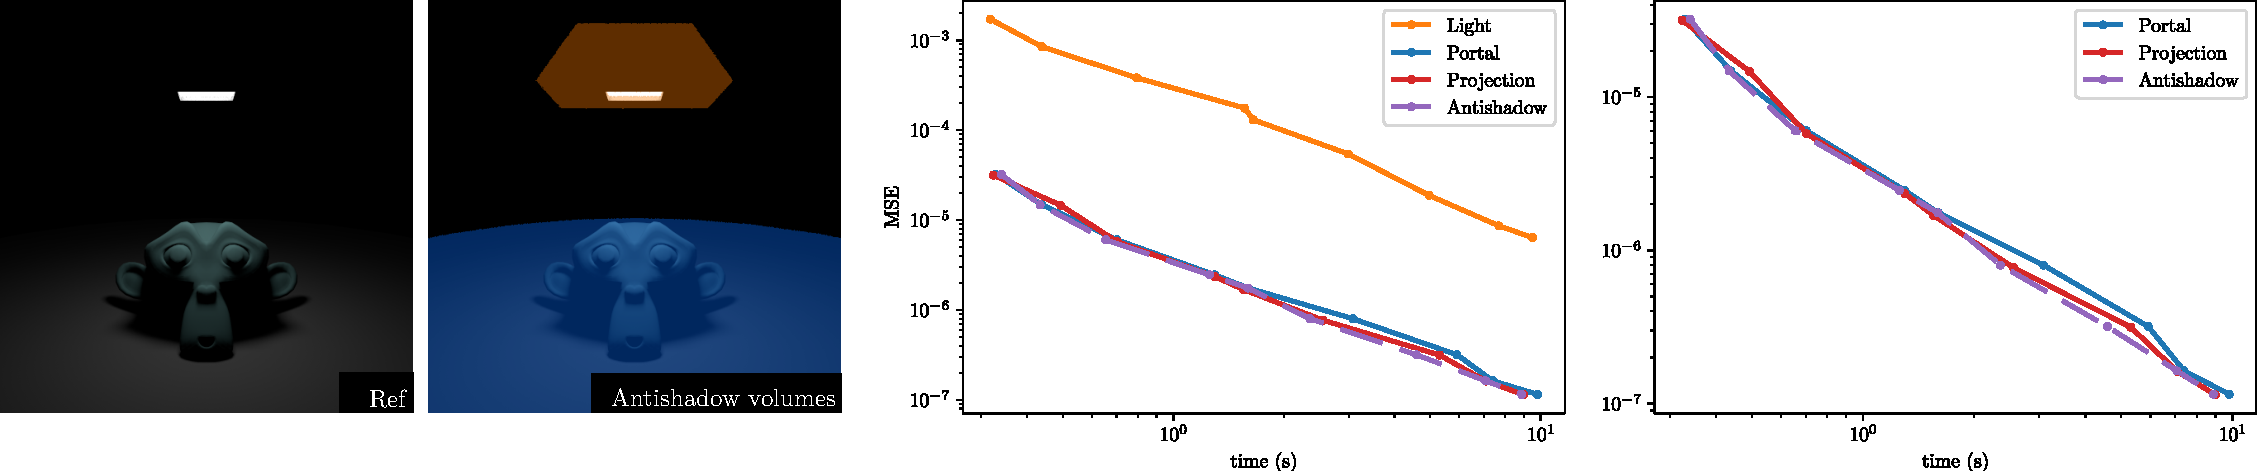
\includegraphics[width=\textwidth]{../pdf/results_a.pdf}
        \label{img:results_small}
    }
    
    \subfloat[\textbf{Small light, large portal:} Optimal sampling strategy is projection.]{
        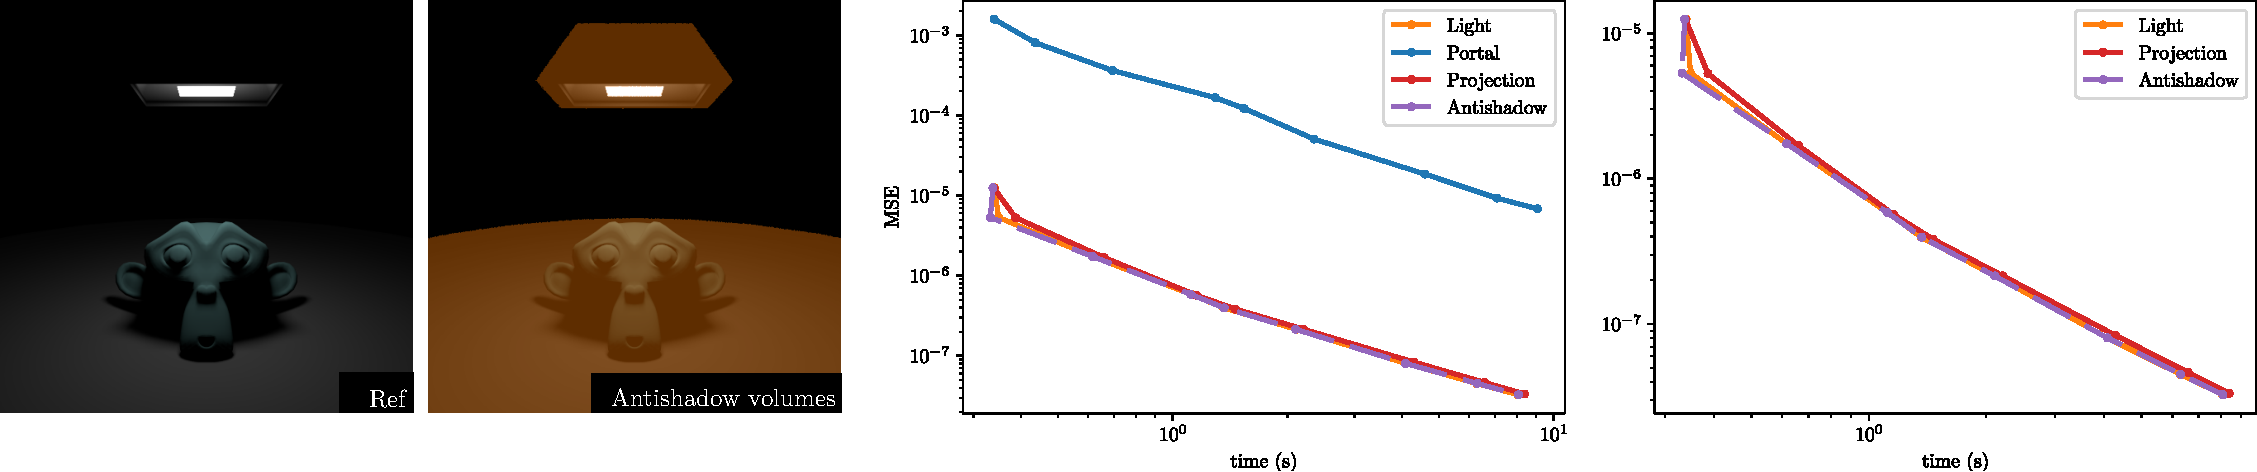
\includegraphics[width=\textwidth]{../pdf/results_b.pdf}
        \label{img:results_big}
    }
    
    \subfloat[\textbf{Balanced light and portal:} Optimal sampling strategy is projection.]{
        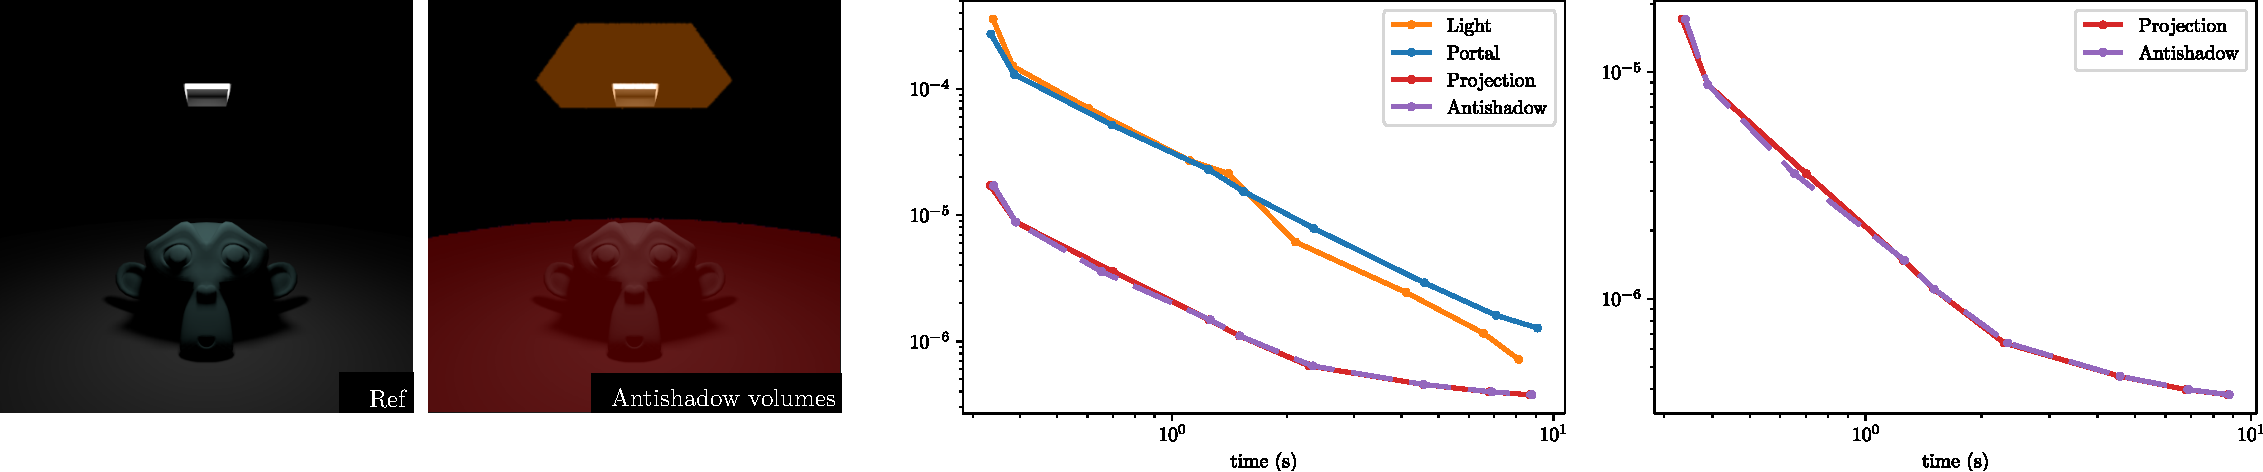
\includegraphics[width=\textwidth]{../pdf/results_c.pdf}
        \label{img:results_balanced}
    }

    \caption{We compare light sampling (baseline), portal sampling, projection sampling and antishadow-based sampling for three \emph{Suzanne} scenes, differing in the portal-light solid angle ratios. Light and portal sampling are not robust as they fail in all scenes but one. Projection sampling works well in all scenes at a small runtime cost, and antishadow-based sampling works as well as projection sampling but at a decreased runtime cost.}
    \label{fig:results}
\end{figure*}



\section{Discussion}
\label{sec:discussion}
\todo[inline, caption={}]{
\begin{minipage}{\linewidth}
    Incomplete due to missing results.\\

    Things to potentially include (depending on if I implement the feature or not):

    \begin{itemize}
        \item \textbf{Limitation:} Requires additional artist input so not great, but mention that since standard light portals are already included in most pipelines it should be feasible to implement it.
        \item \textbf{Limitation:} Method presented is limited to certain combinations of portal shape and light shape, give general guidance on how to generalize
        \item \textbf{Future work:} Multiple portals, decide on which portal to sample based on frustum
        \item \textbf{Future work:} Multiple deciding which portal to sample based on frustum
        \item \textbf{Future work:} Chain portals against eachother and project $i$th portal to $i+1$th portal, good for very precise visibility constraint 
    \end{itemize}
\end{minipage}
}








\section{Conclusion}
\label{sec:conclusion}

\todo[inline]{Incomplete since still on results}

We have developed a strategy for efficiently importance sampling area lights according to the visibility of the light through an artist-specified portal. We demonstrated that the method accelerates convergence for a wide variety of scenes where the light source is partially occluded. 


\printbibliography[heading=bibintoc, title={References}]

\end{multicols*}
\end{document}
